\documentclass[12pt,a4paper,twoside]{article}
\usepackage[left=3.5cm,right=2.5cm,top=1.5cm,bottom=1.5cm,includeheadfoot]{geometry}
\usepackage[onehalfspacing]{setspace}
\usepackage{ngerman}
\usepackage{times}
\usepackage[latin1]{inputenc}
\usepackage[T1]{fontenc}
\usepackage{graphicx}
\usepackage[nottoc,numbib]{tocbibind}
\usepackage{libertine}
\usepackage{microtype}
\usepackage[font=tiny,labelfont=bf]{caption}
\usepackage{listings}
\usepackage{verbatim} 
\usepackage{color}

\renewcommand*{\listoffigures}{%
  \begingroup
  \tocsection
  \tocfile{\listfigurename}{lof}
  \endgroup
}

\definecolor{dkgreen}{rgb}{0,0.6,0}
\definecolor{gray}{rgb}{0.5,0.5,0.5}
\definecolor{mauve}{rgb}{0.58,0,0.82}

\lstset{frame=tb,
	language=C++,
	aboveskip=3mm,
	belowskip=3mm,
	showstringspaces=false,
	columns=fixed,
	basicstyle={\footnotesize\ttfamily},
	numbers=none,
	numberstyle=\tiny\color{gray},
	keywordstyle=\color{blue},
	commentstyle=\color{dkgreen},
	stringstyle=\color{mauve},
	breaklines=true,
	breakatwhitespace=true,
	tabsize=4
}

\begin{document}
	\begin{titlepage}
		\begin{center}
			\huge \bfseries{\scshape{Umsetzung einer objektorientierten Software-Architektur in C++ zur plattformunabh�ngigen Ansteuerung eines Robotermanipulators}} \\  
			\ \\ 
			\ \\
			\LARGE{ 
				\textbf{
					Bachelorarbeit vorgelegt von \\ 
					Willi Penner \\ 
					Matrikelnummer: 1106136 \\
				}
			}
			\ \\
			\ \\
		\end{center}
		\begin{flushleft}
			Angefertigt im Studiengang Mechatronik \\
			(Bachelor of Science, B. Sc.) \\
			\ \\
			Am Fachbereich Ingenierwissenschaften und Mathematik der Fachhochschule Bielefeld \\
			\ \\
			\ \\
			Tag der Abgabe: 24.07.2020 \\
			Sommersemester 2020 \\
			\ \\
			Erstpr�fer: Prof. Dr. rer. nat. Martin H�lse \\
			Zweitpr�fer: Prof. Dr. rer. nat. Axel Schneider \\
		\end{flushleft}    
	\end{titlepage}

	\tableofcontents
		\newpage

	\setcounter{equation}{1} 

	\section{Abstract}
		Text
		\newpage

	\section{Abk�rzungsverzeichnis}
		\begin{tabbing}
    		Links \= Mitte \= \kill
    		Abb. \> \> Abbildung \\
    		ILIAS \> \> \textbf{I}ntegriertes \textbf{L}ern-, \textbf{I}nformations- und \textbf{A}rbeitskooperations-\textbf{S}ystem  \\
   			MEX \> \> \textbf{M}odularer \textbf{Ex}perimentierbaukasten \\
   			$\mu s$ \> \> Mikrosekunden \\
   			$ms$ \> \> Millisekunden \\
  		\end{tabbing}
		\newpage

	\section{Einleitung}
		\sloppy
		Hintergrund dieser Bachelorarbeit ist ein Semesterprojekt aus dem Sommersemester 2019, welches dann im Wintersemester 2019/2020 weitergef�hrt wurde.
		Das Projekt mit dem Namen "`modularer Experementierbaukasten"' (im weiteren Verlauf mit MEX abgek�rzt) hatte zum Ziel einen modularen Roboterbaukasten 
		zu entwickeln, welcher im Rahmen des Moduls Robotik in den Praktika eingesetzt werden soll. Mithilfe des MEX sollen Studierende der Fachhochschule Bielefeld
		erste praktische Erfahrungen in der Roboterprogrammierung sammeln und gelernte Inhalte aus den Vorlesungen in der Praxis anwenden k�nnen. \\
		Die Ergebnisse aus diesem Projekt sowie ihre Dokumentation dienen als Ausgangslage f�r diese Bachelorarbeit. 

		\subsection{Ausgangssituation}
			Zum Beginn der Bachelorarbeit befand sich das zuvor genannte Semesterprojekt kurz vor dem Abschluss. Durch die Projektgruppe ist die Hardware beschafft und 
			die ersten Prototypen aufgebaut worden. Nach der �bergabe der Hardware konnte sowohl der Robotermanipulator als auch eine Teststation f�r die Servomotoren aufgebaut werden.
			Im folgenden ist die f�r die Bachelorarbeit bereitgestellte Hardware gelistet: \\
			\ \\
			Hardware der Teststation
			\begin{itemize}
  				\setlength{\itemsep}{0pt}   
				\item[$\bullet$] Controller: Mini Maestro 12-Channel USB Servo Controller (Abb. \ref{fig:Bild1} auf Seite \pageref{fig:Bild1})
				\item[$\bullet$] Servomotoren: Zwei Micro Servo SG90 (Abb. \ref{fig:Bild2} auf Seite \pageref{fig:Bild2}) 
				\item[$\bullet$] Spannungswandler: DC 7-32V to 0.8-28V Adjustable Step Down Power Supply Module Buck Converter (Abb. \ref{fig:Bild1} auf Seite \pageref{fig:Bild1}) 
			\end{itemize}
 			\begin{figure}[htbp] 
  				\centering
     			\fbox{\includegraphics[width=0.4\textwidth]{bilder/Abbildung_1.png}}
  				\caption{Controller und Spannungswandler (Quelle: eigene Aufnahme)}
  				\label{fig:Bild1}
			\end{figure}
			\begin{figure}[htbp] 
  				\centering
     			\fbox{\includegraphics[width=0.4\textwidth]{bilder/Abbildung_2.png}}
  				\caption{Servomotor SG90 (Quelle: eigene Aufnahme)}
  				\label{fig:Bild2}
			\end{figure}
			Hardware f�r den Robotermanipulator (\ref{fig:Bild3} auf Seite \pageref{fig:Bild3}) 
			\begin{itemize}
  				\setlength{\itemsep}{0pt}   
				\item[$\bullet$] Controller: Mini Maestro 12-Channel USB Servo Controller
				\item[$\bullet$] Servomotoren: Sechs K-Power DM1500 (Abb. \ref{fig:Bild4} auf Seite \pageref{fig:Bild4}) 
				\item[$\bullet$] Diverse mechanische Bauteile f�r den Aufbau des Robotermanipulators 
			\end{itemize}
			\begin{figure}[htbp] 
  				\centering
     			\fbox{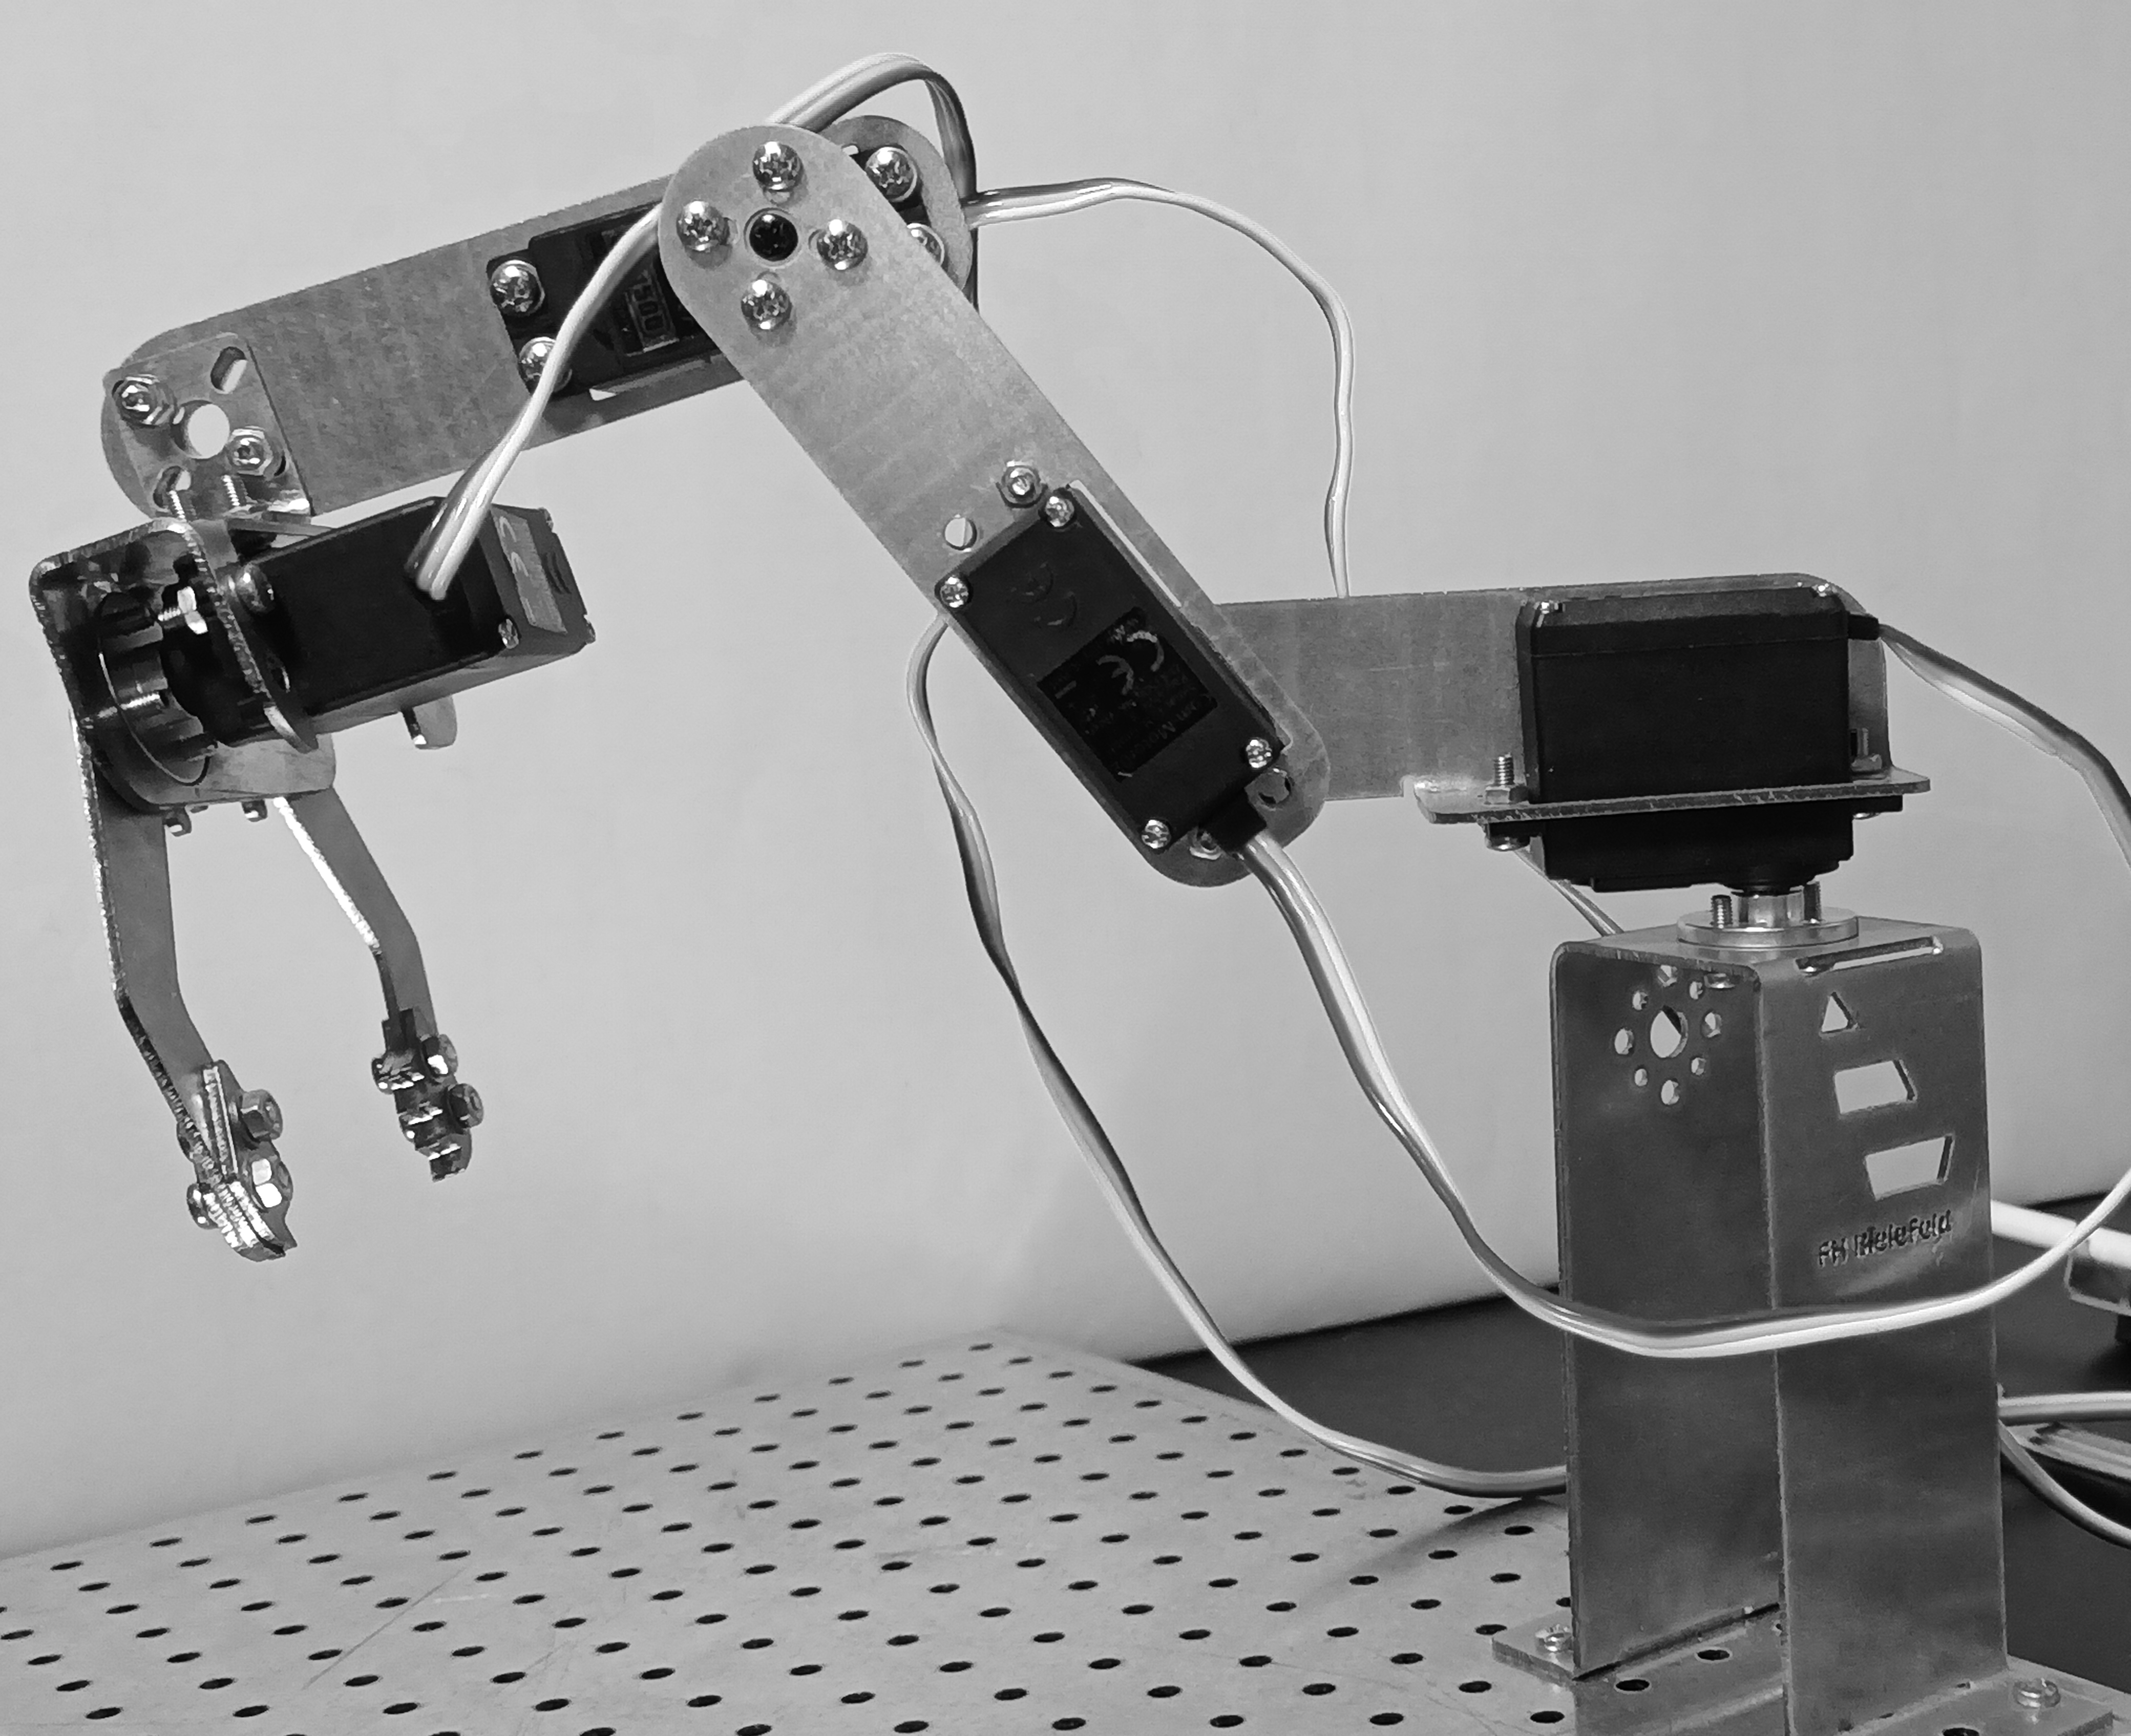
\includegraphics[width=0.4\textwidth]{bilder/Abbildung_3.png}}
  				\caption{Robotormanipulator: Konfiguration mit Greifer (Quelle: eigene Aufnahme)} 
  				\label{fig:Bild3}
			\end{figure}
			\begin{figure}[htbp] 
  				\centering
     			\fbox{\includegraphics[width=0.4\textwidth]{bilder/Abbildung_4.png}}
  				\caption{Servomoter K-Power DM1500 (Quelle: eigene Aufnahme)}  
  				\label{fig:Bild4}
			\end{figure}

		\subsection{Aufgabenstellung}
			Aufgabenstellung der Bachelorarbeit ist die "`Umsetzung einer objektorientierten Software-Architektur 
			in C++ zur plattformunabh�ngigen Ansteuerung eines Robotermanipulators"' f�r die bereits angeschaffte 
			Hardware. Dabei Umfasst die Aufgabenstellung:
			\begin{itemize}
  				\setlength{\itemsep}{0pt}   
				\item[$\bullet$] die Analyse und Erweiterung der durch die Projektgruppe erstellte Software-Architektur 
				\item[$\bullet$] Implementieren der Schnittstelle zur Ansteuerung des Robotermanipulators unter Windows
				\item[$\bullet$] Portieren der Schnittstelle nach Linux
				\item[$\bullet$] Testen der Schnittstelle an der Teststation und am Robotormanipulator sowohl unter Windows als auch unter Linux
			\end{itemize}  

		\subsection{Projektorganisation}
			F�r die Projektbetreuung ist zu Beginn ein w�chentliches Projektmeeting festgelegt worden. Die Meetings dienten dem Projekt
			zugrunde liegenden interativen Entwicklungsprozess. Das bedeutet das sich die Aufgabenstellung von Meeting zu Meeting weiterentwickelt hat. \\
			Um die sich entwickelnde Aufgabenstellung zu dokumentieren ist im ILIAS ein Forum eingerichtet worden. Zus�tzlich existiert dort ein Ordner um 
			Projektdateien hochladen zu k�nnen. \\
			Unter GitHub ist f�r die programmierten Sourcefiles ein Repository eingerichtet. Dies dient sowohl dem verfolgen des Projektfortschritts 
			durch den Projektbetreuer als auch der Datensicherung des Quellcodes.

	\section{Analyse der Software-Architektur}
		\begin{figure}[htbp] 
  			\centering
     		\fbox{\includegraphics[width=0.9\textwidth]{bilder/Abbildung_5.png}}
  			\caption{UML-Diagramm der Software-Architektur (Quelle: Projektdokumentation MEX-Projekt)}  
  			\label{fig:Bild5}
		\end{figure}
		\noindent Der Abbildung \ref{fig:Bild5} auf Seite \pageref{fig:Bild5} zeigt das UML-Diagramm der Software-Architektur, welches die
		Projektgruppe aus dem Wintersemester 2019/2020 erstellt hat. Bei dem Vergleich des UML-Diagramms und des Quellcodes ist 
		festgestellt worden, das diese sich signifikant Unterscheiden. \\
		Das UML-Diagramm sieht eine Klasse "`Pololu"' vor, die durch Vererbung die Methoden der Klassen "`IPololu"' und "`ISerialCom"' erh�lt. Diese
		werden dann wiederrum an die Klasse "`StandardManip.A"' vererbt. Die Klasse "`StandardManip.A"' bietet dem Nutzer die Funktionen eine serielle Verbindung
		zu �ffnen, zu Schlie�en und Positionswerte f�r eine Servomotor zu setzen. \\
		Die Namen "`IPololu"' und "`ISerialCom"' suggerieren, dass es sich um Interface-Klassen handelt, dabei handelt es sich um einfache Klassen. Aus dem UML-Diagramm
		ist ebenfalls nicht ersichtlich welche Klassen Attribute enthalten bzw. welche �bergabeparameter die einzelnen Funktionen haben.
		Im Quellcode ist lediglich die Klasse "`IPololu"' umgesetzt, sie enth�lt die Funktionen um Positionswerte von angeschlossenen Servomotoren zu ver�ndern: \\
		
		\begin{lstlisting}{IPololu_OLD}
			unsigned char setTarget(HANDLE port, unsigned char channel,unsigned short target)
			unsigned char setMultipleTargets(HANDLE port, unsigned char numberoftargets, unsigned char channel, unsigned short target)
		\end{lstlisting}
		
		 
		
	\section{A}
		Text

	\section{D}
		Text
		\newpage

	% Abbildungsverzeichnis
	\listoffigures
		\newpage

	%Eidesstattlische Versicherung
	\section{Eidesstattliche Versicherung}
		Ich erkl�re hiermit an Eides Statt, dass ich die vorliegende Arbeit selbst�ndig und ohne 
		Benutzung anderer als der angegebenen Hilfmittel angefertigt habe. Die aus fremden Quellen 
		direkt oder indirekt �bernommenen Gedanken sind als solche kenntlich gemacht. \\
		\ \\
		\ \\
		\ \\
		\ \\
		\_\_\_\_\_\_\_\_\_\_\_\_\_\_\_\_\_\_\_\_\_\_\_\_ \\ 
		(Willi Penner) \\
		\newpage

	\section{Anhang}
		Text

\end{document}
